\section{Introdução Teórica}

Esta secção serve de introdução teórica aos conceitos utilizados ao longo do relatório. O objectivo é relembrar o fundamental e establecer a terminologia a utilizar no desenvolvimento do relatório.

% ---------------------- Message Oriented Middleware
\section{Message Oriented Middleware - MoM}
Um \textit{Message Oriented Middleware}, ou simplesmente MoM é uma arquitectura que fornece uma camada entre as aplicaçães, substituindo a comunicação directa entre as mesmas por um sistema de troca de mensagens.\\
Uma implementação \textit{MoM} oferece uma API capaz de funcionar com um número relativamente vasto de plataformas e redes. Essa API fornece um nível de abstracção capaz de aumentar a portbailidade, interoperabilidade e flexibilidades das aplicações que correm sobre a MOM.\\
Usando a API, os programadores são libertados dos detalhes das várias plataformas e protocolos, reduzinhdo assim a complexidade da implementação das comunicações das suas aplicações.\\
A comunicação é efectuada através de mensagens que são transmitidas, ou pela estrutura típica cliente/servidor(usando \textit{broadcast} ou \textit{multicast}), ou entre pilhas mantidas por gestores locais. A alternativa que usa gestores de pilhas é a mais poderosa em termos de aplicabilidade e versatilidade.\\ 
Os sistemas que usam MOM providencias comunicação distribuída com base num modelo d einteracção assíncrono. Os participantes do sistema não precisam de bloquear e espearar numa mensagem enviada, eles podem continuar a processar assim que uma mensagem for enviada. Isso permite a entrega de mensagens quando o receptor ou emissor não estejam activos ou disponíveis para responder na altura da execução. Uma aplicação que envia mensagens não tem a garantia que a sua mensagem vai ser lida por outra aplicação, nem sequer tem a garantia de quanto tempo vai demorar até que a sua mensagem seja entregue. 
\subsection{Modelos de Mensagens}
\subsubsection{Ponto a Ponto}
O modelo de mensagens ponto a ponto fornece uma troca assíncrona de mensagens entre aplicações. Neste modelo, as mensagens de um cliente produtor são encaminhadas para um cliente consumidor através de uma \textit{queue}. O mecanismo mais comun de \textit{queue} é uma \textit{queue} FIFO, na qual as mensagens são ordenadas conforme a ordem em que são recebidas pelo sistema de mensagens, assim que são consumidas são removidas do topo da \textit{queue}. 
Enquanto não existe uma restrição para o número de clientes que podem publicar numa \textit{queue}, existe normalmente apenas um cliente consumidor, apesar de não ser um requisito muito rígido. Cada mensagem que é entregue apenas uma vez a apenas um receptor. o modelo permite que múltiplos receptores possam se concetar à queue, mas epnas um dos receptores vai consumir a mensagem. As técnicas de usar múltiplos clientes para ler de uma \textit{queue} pode  
\subsubsection{Publish/Subscribe}
O mecanismo  de \textit{Publish/Subscribe} é um mecanismo muito poderoso, usado para desiminar informação entre produtores e consumidores anonímos de mensagens. Podem ser relaçoes de um para um ou de muitos para muitos, permitem a uma simples consumidas enviar e receber mensagens de potencilamente centenas de milhares de utilizadores. \\
No modelo publish



\subsection{Message Broker}
A definição mais aceite de um broker de um \textit{Message Broker} é a de um software de alto nível que lida com problemas relacionados com a integração da aplicação. É tipicamente construído sobre um MOM, que providencia a base da comunicação entre as aplicações, persistência de mensagens e garantias de entrega. Modelos de \textit{Message Broker}:
\begin{itemize}
\item \textbf{Com broker} O modelo tradicional de MOM que utiliza um broker. Funciona como uma arquitectura em estrela em que todas as aplicações são ligadas através do broker e nenhuma comunicação é feita directamente. Dessa maneira as aplicações não tem necessidade de ter conhecimento da localização umas das outras, apenas o endereço do broker. A comunicação não exige que elas coexistam no espaço e no tempo além do broker ser independente das aplicações. Este mecanismo exige no entanto uma imensa troca de mensagens pela rede e todas tem de passar pelo broker podendo a levar a que se torne num \textit{bottleneck} do sistema.
\begin{figure}[H]
\centering
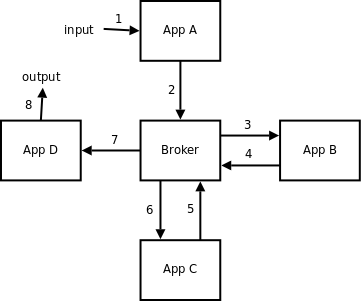
\includegraphics[width=0.65\textwidth]{broker1.png}
\caption{\textit{Arquitectura com Broker}}
\label{fig:broker}
\end{figure}
\item \textbf{Sem broker}\\
A imagem mostra um cenário em que não existe broker.
\begin{figure}[H]
\centering
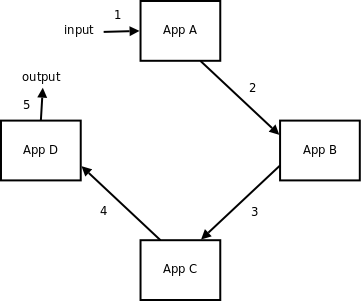
\includegraphics[width=0.65\textwidth]{nobroker.png}
\caption{\textit{Arquitectura sem Broker}}
\label{fig:nobroker}
\end{figure}
O número de mensagens decresce e não existe nenhum tipo de limitação do género \textit{bottleneck} como no exemplo anterior. Este tipo de arquitectura é ideal para sistemas com exigências de baixa latência de comunicação e com alta taxa de transacções. Cada aplicação apenas tem de se conectar com a aplicação ou aplicações com que faz a comunicação, tendo de saber o endereço de cada uma delas. Apesar de ser aceitável neste exemplo simples,  No  mundo real não tem aplicação porque nesses casos existem centenas de milhares de aplicações ligadas. Fazer a gestão dessas ligações todas seria um trabalho muito custoso.\\
\item \textbf{Broker como serviço de Directorias} \\
A funcionalidade do broker pode ser dividida em duas partes separadas. Primeiro, o broker como um repositório de aplicações a correr na rede. Sabe que a aplicação X corre num host Y e que as mensages para X devem ser mandadas para Y. Age como um serviço de directorias. Segundo, o broker faz a troca de mensagens ele mesmo.\\
Para resolver problemas de gestão, a tarefa de troca de mensagens pode ser feita pelas aplicações. Uma aplicação X pode registar ao broker que corre no host Y. A aplicação Z quer envias uma mensagem para a aplicação X vai "questionar" o broker sobre a localização de X. Assim que a resposta de que X está em Y chegar a Z, Z pode criar uma conecção directa para Y e enviar a mensagem por ele mesmo sem incomodar o broker. A imagem em baixo ilustra a arquitectura:\\
\begin{figure}[H]
\centering
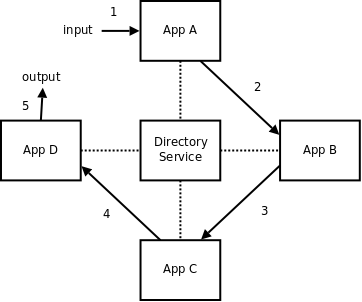
\includegraphics[width=0.65\textwidth]{dsbroker.png}
\caption{\textit{Broker como Serviço de directorias}}
\label{fig:dsbroker}
\end{figure}
Dessa maneira é possível obter uma maior performance e tornar o sistema mais fácil de gerir ao mesmo tempo.
\item \textbf{Broker Distribuído}\\
Para atingir o tipo de comportamento suposto para um \textit{Message Broker} é apenas necessário um broker no meio, mas não é possível evitar o problema do broker como \textit{bottleneck}. Uma arquitectura distribuída evita esse problema.\\
\begin{figure}[H]
\centering
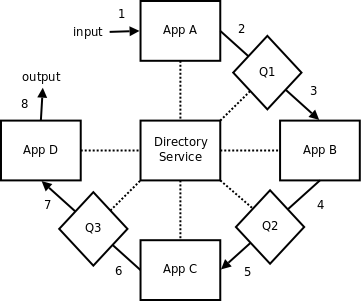
\includegraphics[width=0.65\textwidth]{dbroker.png}
\caption{\textit{Broker distribuído}}
\label{fig:distributedbroker}
\end{figure}
Como podemos ver pela imagem, cada fila de mensagen é implementada como aplicação separada. Pode correr no mesmo host que aplicação a que esta ligado ou pode correr num host completamente diferente. Muitas filas podem correr num simples host, o host pode ser dedicado exclusivamente a ter apenas uma fila. A fila é registada com o broker e assim é acessível a todas as aplicações na rede. A fila é uma peça de software bastante simples que recebe mensagens dos emissores e distribui pelos receptores. A change de falhar é bastante mais baixa que aplicações reais cheias de complexidade de negócio.
\end{itemize}




% ---------------------- Websockets
\input{websockets}

\subsection{Ruby}
\label{sec:ruby}

Ruby é uma linguagem de programação intrepertada com suporte para diferentes paradigmas (funcional, orientado a objectos e imperativo). Desde o lançamento em 1995 Ruby tem crescido em comunidade e potencial. O seu criador, Yukihiro Matsumoto, pretendia uma linguagem que qualquer programador pudesse aperciar:

\begingroup
\leftskip4em
\rightskip\leftskip
``Ruby is simple in appearance, but is very complex inside, just like our human body.'' \cite{matz}
\par
\endgroup

Ruby encontra-se actualmente na versão 2.0.0-p195 no entanto o projecto foi desenvolvido na versão \textbf{2.0.0p0}.

\subsubsection{\textit{Global Interpreter Lock}}
\label{sec:gil}

Existem diversos intrepertadores para Ruby sendo os mais importantes \textbf{Matz's Ruby Interpreter (MRI)}, em homenagem ao criador, e \textbf{JRuby}, implementado no topo da Java Virtual Machine.
A diferença mais relevante entre ambos para este projecto é o \textit{Global Interpreter Lock} (GIL) que existe no MRI. O GIL é uma camada responsável por proteger o intrepertador contra código \textit{non thread-safe}.

A figura~\ref{fig:ruby-gil} apresenta uma comparação entre três versões do Ruby. Na versão 1.8 o intrepertador Ruby possuí apenas uma thread do sistema para execussão. Já na versão 1.9, e também na versão 2 ainda que não seja visível na imagem, várias threads do sistema são alocadas ao intrepertador, o que parece prometer paralelismo de execussão. No entanto em ambos os casos existe a camada do GIL que protegendo contra a execussão de código \textit{non thread-safe} permite que apenas uma thread seja executada de cada vez pelo processador, ou seja, ambas as versões do Ruby correm num core do CPU apenas.
Por outro lado a implementação em JRuby não contém a camada GIL o que abre as portas ao paralelismo das aplicações em Ruby.

\begin{figure}[H]
\centering
\includegraphics[width=0.9\textwidth]{xruby_gil.png}
\caption{\textit{Global Interpreter Lock}}
\label{fig:ruby-gil}
\end{figure}

Parecendo um cenário desvantajoso para o MRI é de notar que existem soluções para contornar este problema. Se se pensar em processos em vez de threads por procurar-se outros meios de repartir trabalho. Decompondo a aplicação e adicionando meios de comunicação entre processos (Starling, RabbitMQ, outros) consegue-se que multiplos processos da mesma aplicação executem concurrentemente.
